% !TeX program = xelatex
% This approved increment covers textbook sections 1.1 through 1.4 only.
\documentclass[12pt,a4paper]{article}
\RequirePackage{array}[=2024-06-01]
% !TeX root = ../2/main.tex
\usepackage[a4paper,margin=25mm,headheight=16pt]{geometry}
\usepackage{amsmath,amssymb}
\usepackage{graphicx}
\usepackage{booktabs}
\usepackage{tabularx}
\usepackage{siunitx}
\usepackage{tikz}
\usepackage{circuitikz}
\usepackage[unicode,hidelinks]{hyperref}
\usepackage{xepersian}
% Only the regular B Nazanin file is installed; synthesize bold explicitly.
\settextfont[Path=C:/Windows/Fonts/,AutoFakeBold=2,AutoFakeSlant=0.2]{B-NAZANIN.TTF}
% B Nazanin lacks U+066A (Arabic percent), required by xepersian's digit setup.
% Arial covers the complete required digit/punctuation set; Persian prose remains B Nazanin.
\setdigitfont[Path=C:/Windows/Fonts/,BoldFont=arialbd.ttf,ItalicFont=ariali.ttf,BoldItalicFont=arialbi.ttf]{arial.ttf}
\setmathdigitfont[Path=C:/Windows/Fonts/,BoldFont=arialbd.ttf,ItalicFont=ariali.ttf,BoldItalicFont=arialbi.ttf]{arial.ttf}
\setlatintextfont{TeX Gyre Termes}
% B Nazanin does not contain the default itemize bullet and dash glyphs.
\renewcommand{\labelitemi}{\(\bullet\)}
\renewcommand{\labelitemii}{\(\circ\)}
\renewcommand{\labelitemiii}{\(\diamond\)}
\setlength{\parindent}{0pt}
\setlength{\parskip}{0.5em}
\linespread{1.25}
\newcommand{\exercise}[1]{\section*{تمرین #1}}
% !TeX root = ../2/main.tex
% Shared title page for every assignment.
% Change only \AssignmentNumber and \AssignmentDate in each main document.

\newcommand{\AssignmentNumber}[1]{\gdef\assignmentnumber{#1}}
\newcommand{\AssignmentDate}[1]{\gdef\assignmentdate{#1}}

\newcommand{\assignmentnumber}{---}
\newcommand{\assignmentdate}{---}

% Stable course metadata
\newcommand{\universityname}{دانشگاه صنعتی امیرکبیر}
\newcommand{\universityalias}{پلی‌تکنیک تهران}
\newcommand{\facultyname}{دانشکده مهندسی کامپیوتر}
\newcommand{\coursename}{طراحی مدارهای مجتمع پرتراکم پیشرفته}
\newcommand{\studentname}{محمد خلیلی اصل}
\newcommand{\instructorname}{دکتر مهدی صدیقی}

\newcommand{\MakeAssignmentCover}{%
  \begin{titlepage}
    \thispagestyle{empty}
    \centering
    \linespread{1}\selectfont

    \vspace*{0mm}
    
\includegraphics[width=44mm]{assets/aut-logo-black.png}\par
    \vspace{3mm}

    {\Large\bfseries \universityname\par}
    \vspace{1mm}
    {\large (\universityalias)\par}
    \vspace{1mm}
    {\large \facultyname\par}

    \vspace{8mm}
    {\Large\bfseries درس \coursename\par}

    \vspace{12mm}
    {\large عنوان\par}
    \vspace{2mm}
    {\LARGE\bfseries تمرین شماره \assignmentnumber\par}

    \vspace{10mm}
    {\large تهیه‌کننده\par}
    \vspace{2mm}
    {\Large\bfseries \studentname\par}

    \vspace{10mm}
    {\large استاد درس\par}
    \vspace{2mm}
    {\Large\bfseries \instructorname\par}

    \vspace{10mm}
    {\Large \assignmentdate\par}
    \vfill
  \end{titlepage}
  \setcounter{page}{1}%
}


\XeTeXgenerateactualtext=1
\newcommand{\secnum}[1]{\mbox{\beginL#1\endL}}
\setlength{\emergencystretch}{3em}
\AtBeginDocument{\DeclareSIPrefix{\micro}{\text{\lr{µ}}}{-6}}
\widowpenalty=10000
\clubpenalty=10000
\hypersetup{pdftitle={جزوه اول؛ معرفی VLSI و منطق CMOS}}
\AssignmentNumber{جزوه اول؛ معرفی و منطق \lr{CMOS}}
\AssignmentDate{بخش‌های \secnum{۱.۱} تا \secnum{۱.۴} کتاب}
\patchcmd{\MakeAssignmentCover}{تمرین شماره \assignmentnumber}{\assignmentnumber}{}{\errmessage{Cover title replacement failed}}
\begin{document}
\MakeAssignmentCover
\section*{مسیر مطالعه و محدوده این بخش}
در بخش پیش‌نیازها، کمیت‌های مدار، قوانین گره و حلقه، خازن و عملگرهای منطقی
آموزش داده شدند. اکنون می‌خواهیم ببینیم این عملگرها چگونه از ترانزیستور ساخته می‌شوند.
ابتدا انگیزه \lr{VLSI} و ساختار مقدماتی \lr{MOS} معرفی می‌شود؛ سپس مسیر
\lr{Inverter}، گیت‌های چندورودی، انتخاب داده و ذخیره یک بیت را دنبال می‌کنیم.

این فایل، بخش‌های \secnum{۱.۱} تا \secnum{۱.۴} کتاب مرجع را پوشش می‌دهد
\cite{weste}. جزوه کامل فصل اول یا تحلیل کمی فصل دوم هنوز نیست.
برای کنترل جهت و معنای روابط، هر شرط هدایت از تابع خروجی جدا نوشته می‌شود.
مثال‌های تکمیلی و نمودارهای آموزشی این جزوه، نتیجه شبیه‌سازی یا داده یک فناوری نیستند.
شکل‌های مداری بازترسیم آموزشی‌اند؛ اتصال‌هایشان باید همراه با توضیح متن خوانده شود.

اسلاید \lr{00} مدل \lr{Switch} و گیت‌های پایه را عرضه می‌کند؛
موضوعات پیشرفته‌تر بخش \secnum{۱.۴} از کتاب تکمیل شده‌اند.
اشاره اسلاید به لایه‌های طراحی در اینجا فقط مقدمه است؛ بخش‌های \secnum{۱.۵}
تا \secnum{۱.۱۲} در گام بعدی جزوه اول خواهند آمد.
\tableofcontents
\clearpage
% !TeX root = booklet-01.tex
\section{از مدار مجتمع تا \lr{VLSI}}
\label{sec:ch1-history}
\subsection{چرا مجتمع‌سازی اهمیت دارد؟}
در \lr{Integrated Circuit (IC)}، تعداد زیادی قطعه و اتصال روی یک بستر
ساخته می‌شوند. این کار با کنار هم قرار دادن قطعات مجزا روی برد تفاوت دارد:
ابعاد اجزا و فاصله اتصال‌ها می‌توانند بسیار کوچک‌تر باشند و ساخت تعداد زیادی
قطعه با یک فرایند تکرارشونده امکان‌پذیر می‌شود.
اصطلاح \lr{Very Large-Scale Integration (VLSI)} به مجتمع‌سازی در مقیاس بسیار
بزرگ اشاره دارد. مرزهای نام‌گذاری تاریخی \lr{SSI}، \lr{MSI} و \lr{LSI}
رده‌بندی سخت و همیشگی همه تراشه‌ها نیستند؛ کتاب از \lr{VLSI} به‌عنوان نام رایج
مدارهای با مجتمع‌سازی گسترده یاد می‌کند \cite[بخش \secnum{۱.۱}]{weste}.

مطابق روایت تاریخی کتاب، ترانزیستور نقطه‌تماسی در ۱۹۴۷ به دست
\lr{John Bardeen} و \lr{Walter Brattain} ساخته شد و نمونه نخست \lr{IC}
را \lr{Jack Kilby} در ۱۹۵۸ ساخت.
ترانزیستورهای \lr{Bipolar} در مدارهای اولیه نقش مهمی داشتند؛
در مقابل، \lr{MOSFET} با \lr{Gate} عایق‌شده، جریان کنترلی رسانشی بسیار کمی
در حالت ساکن نیاز دارد. ترکیب \lr{nMOS} و \lr{pMOS} به منطق \lr{CMOS}
با توان ساکن پایین در مدل ایدئال می‌انجامد
\cite[صفحات چاپی ۱ تا ۳]{weste}\cite[اسلایدهای ۴ تا ۸]{intro}.
این به معنی صفر بودن جریان هنگام شارژ ظرفیت \lr{Gate} یا نبود \lr{Leakage} واقعی نیست.

\subsection{رشد نمایی و \lr{Moore's Law}}
اگر تعداد ترانزیستورها در هر بازه زمانی یکسان دو برابر شود، رشد نمایی داریم.
با \(N_0\) تعداد اولیه، \(T\) زمان دو برابر شدن و \(t\) زمان سپری‌شده، مدل آموزشی زیر را می‌نویسیم:
\begin{equation}\label{eq:ch1-doubling}
N(t)=N_0\,2^{t/T}.
\end{equation}
نسبت \(t/T\) بدون واحد است. در \(t=0\)، ضریب رشد یک است؛ در \(t=T\)
دو و در \(t=2T\) چهار می‌شود. در رشد خطی، افزایش مطلق در بازه‌های برابر ثابت است؛
در این مدل نمایی، ضریب افزایش ثابت است.

\textbf{مثال آموزشی.} فرض کنیم \(N_0=1000\) و \(T\) دو سال باشد.
پس از شش سال، \(t/T=3\) و \(N=1000\times2^3=8000\).
این مثال پیش‌بینی صنعت یا تعداد واقعی ترانزیستورهای یک محصول نیست.

کتاب، \lr{Moore's Law} را به روند تاریخی افزایش تعداد ترانزیستورهای قابل ساخت
اقتصادی مرتبط می‌کند و برای داده‌های پردازنده‌های \lr{Intel} در شکل
\secnum{۱.۴} خود، زمان دو برابر شدن حدود ۲۶ ماه را گزارش می‌کند.
این برازش تاریخی، قانون بنیادی طبیعت یا تضمین یک دوره ثابت برای همه فناوری‌ها نیست
\cite[صفحات چاپی ۳ و ۴]{weste}\cite[اسلاید ۹]{intro}.
آمار و پیش‌بینی‌های کتاب و اسلاید متعلق به دوره انتشارشان هستند؛
در این جزوه به‌عنوان وضعیت فعلی صنعت گزارش نمی‌شوند.

اسلاید ۵، نرخ رشد مرکب سالانه تاریخی ۵۳ درصد را برای بازه مورد بحث خود ذکر
می‌کند \cite{intro}. اگر نرخ سالانه ثابت \(r\) باشد و \(t\) بر حسب سال سنجیده
شود، مدل رشد \(N(t)=N_0(1+r)^t\) است.
با \(r=0.53\)، پس از دو سال ضریب رشد \((1.53)^2=2.3409\) می‌شود.
افزایش سال دوم بر مقدار افزایش‌یافته سال اول اعمال می‌شود.
این گزارش تاریخی و برازش ۲۶ماهه شمار ترانزیستورهای نمونه‌های \lr{Intel}،
به مجموعه داده و بازه خود مربوط‌اند.

\subsection{چرا نمودار نیمه‌لگاریتمی می‌تواند خطی باشد؟}
لگاریتم، توان لازم برای رسیدن به یک عدد از یک پایه را نشان می‌دهد.
مثلاً \(\log_2 8=3\)، چون \(2^3=8\).
با گرفتن لگاریتم پایه دو از رابطه \eqref{eq:ch1-doubling}، برای \(N,N_0>0\)، داریم:
\begin{equation}\label{eq:ch1-semilog}
\log_2 N(t)=\log_2 N_0+\frac{t}{T}.
\end{equation}
از قاعده \(\log_2(ab)=\log_2 a+\log_2 b\) و
\(\log_2(2^x)=x\) استفاده شد.
در نموداری که محور زمان معمولی و محور تعداد لگاریتمی است، رشد نمایی ایدئال
به خط راست تبدیل می‌شود؛ فاصله‌های برابر روی محور لگاریتمی نسبت‌های برابر را نشان می‌دهند،
نه اختلاف‌های برابر. این نکته روش خواندن نمودار تاریخی کتاب را روشن می‌کند.

\subsection{کوچک‌تر شدن، مساحت، توان و محدودیت‌ها}
اگر در یک مدل هندسی ساده هر دو بعد افقی یک قطعه در \(s\) ضرب شوند،
مساحت آن در \(s^2\) ضرب می‌شود. برای \(s=0.7\)، مساحت نسبی \(0.49\) است؛
در مساحت ثابت تراشه و با فرض ثابت بودن سایر محدودیت‌ها، ظرفیت هندسی تعداد قطعات
حدود \(1/0.49\approx2.04\) برابر می‌شود. این استدلال علت ارتباط
کاهش ابعاد و افزایش چگالی را توضیح می‌دهد؛ فضای سیم‌ها، تماس‌ها و محدودیت‌های طراحی را حذف کرده است.

کتاب در بحث \lr{Scaling}، محدودیت توان، نشتی و هزینه طراحی را نیز بیان می‌کند
\cite[صفحات چاپی ۴ تا ۶]{weste}.
بنابراین افزایش تعداد ترانزیستورها لزوماً به همان نسبت فرکانس یا کارایی برنامه را افزایش نمی‌دهد.
\lr{Delay}، \lr{Power} و \lr{Area} معیارهای متفاوتی‌اند و انتخاب یک مدار
ممکن است میان آن‌ها موازنه ایجاد کند. تحلیل کمی این موازنه‌ها به مدل جریان و ظرفیت نیاز دارد.

\section{پیش‌نمایش مسیر طراحی}
\label{sec:book-preview}
تابع منطقی، مدار ترانزیستوری و شکل فیزیکی سه توصیف متفاوت از یک طراحی‌اند.
مثلاً \(Y=\overline{A}\) تابع است؛ دو ترانزیستور با اتصال مشخص، مدار آن است؛
و ناحیه‌های مواد و اتصال‌ها، \lr{Layout} آن را می‌سازند.
استفاده از ابزارهای خودکار، نیاز به فهم این رابطه‌ها را از بین نمی‌برد؛
کتاب به همین دلیل مسیر آموزش را از مدل‌های ساده مدار آغاز می‌کند
\cite[بخش \secnum{۱.۲}]{weste}.
در ادامه، منطق و ذخیره یک بیت، فرآیند ساخت و سطوح طراحی بررسی می‌شوند.

\section{ساختار مقدماتی \lr{MOS Transistor}}
\label{sec:ch1-mos}
\subsection{از \lr{Silicon} به حامل بار}
\lr{Silicon} یک نیمه‌هادی با شبکه بلوری است؛ الکترون‌های لایه ظرفیت آن
در پیوند با اتم‌های مجاور شرکت می‌کنند. افزودن مقدار کنترل‌شده ناخالصی
را \lr{Doping} می‌نامیم. در \lr{n-type}، الکترون‌ها حامل غالب و در
\lr{p-type}، حفره‌ها یا \lr{Hole} حامل غالب‌اند
\cite[بخش \secnum{۱.۳}]{weste}\cite[اسلایدهای ۲ و ۳]{mos}.

\lr{Hole} اتم جداگانه‌ای نیست؛ نبود یک الکترون در پیوند است که با جابه‌جایی
الکترون‌های مجاور، مانند حامل بار مثبت جابه‌جا می‌شود.
نام‌های \lr{n-type} و \lr{p-type} به نوع حامل غالب اشاره دارند؛
به معنی منفی یا مثبت بودن بار خالص کل توده نیمه‌هادی در حالت معمول نیستند.

وقتی ناحیه \lr{p-type} و \lr{n-type} کنار هم قرار گیرند، پیوند \lr{PN}
تشکیل می‌شود. بایاس مستقیم آن، یعنی پتانسیل سمت \lr{p} نسبت به سمت \lr{n}
به‌اندازه کافی بالاتر باشد، امکان جریان قابل‌توجه را فراهم می‌کند؛
در بایاس معکوس معمول، جریان کوچک است.
این توضیح به معنی وجود یک ولتاژ آستانه دقیق و همگانی برای همه دیودها نیست؛
شکست در بایاس معکوس زیاد نیز خارج از مدل مقدماتی است
\cite[صفحه چاپی ۷]{weste}.

\subsection{چهار پایانه و نقش عایق}
\lr{Metal-Oxide-Semiconductor Field-Effect Transistor (MOSFET)}
چهار پایانه دارد: \lr{Gate}، \lr{Source}، \lr{Drain} و \lr{Body}.
\lr{Gate} از نیمه‌هادی با لایه عایق جدا می‌شود.
در مدل مقدماتی، میدان ناشی از ولتاژ \lr{Gate} تعداد حامل‌ها نزدیک سطح
را تغییر می‌دهد و مسیر میان \lr{Source} و \lr{Drain} را کنترل می‌کند.
پس \lr{Gate} ورودی کنترل است، نه سیمی که جریان اصلی از آن وارد خروجی شود.

شکل \ref{fig:ch1-crosssection} یک مقطع ساده \lr{nMOS} است؛ مقیاس واقعی ندارد.
در این مقطع، دو ناحیه \(n^+\) در بدنه \lr{p-type} قرار دارند؛
علامت مثبت در \(n^+\) یعنی \lr{Doping} زیاد، نه بار مثبت ناحیه.
جزئیات اتصال بدنه و ساخت آن در بخش \secnum{۱.۵} آموزش داده می‌شود.
\begin{figure}[ht]
\centering
\begin{latin}
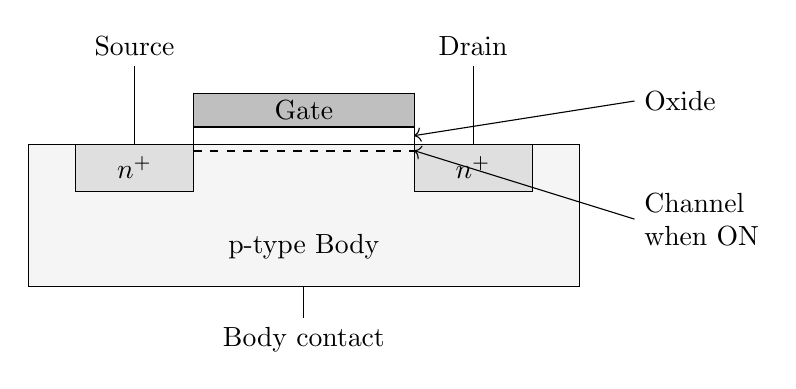
\begin{tikzpicture}[x=1cm,y=1cm]
\draw[fill=gray!8] (0,0) rectangle (7,1.8);
\draw[fill=gray!25] (0.6,1.2) rectangle (2.1,1.8);
\draw[fill=gray!25] (4.9,1.2) rectangle (6.4,1.8);
\node at (1.35,1.5) {$n^+$};\node at (5.65,1.5) {$n^+$};
\node at (3.5,0.5) {p-type Body};
\draw[fill=white] (2.1,1.8) rectangle (4.9,2.02);
\draw[fill=gray!50] (2.1,2.02) rectangle (4.9,2.45);
\node at (3.5,2.23) {Gate};
\draw (1.35,1.8)--(1.35,2.8) node[above] {Source};
\draw (5.65,1.8)--(5.65,2.8) node[above] {Drain};
\draw (3.5,0)--(3.5,-0.4) node[below] {Body contact};
\draw[<-] (4.9,1.91)--(7.7,2.35) node[right] {Oxide};
\draw[dashed,thick] (2.1,1.72)--(4.9,1.72);
\draw[<-] (4.9,1.72)--(7.7,0.85) node[right,align=left] {Channel\\when ON};
\end{tikzpicture}
\end{latin}
\caption{طرح آموزشی مقطع \lr{nMOS} بر پایه شکل \secnum{۱.۹} کتاب
\cite{weste}. خط‌چین محل تشکیل کانال را نشان می‌دهد؛ وجود همیشگی کانال را القا نمی‌کند.
خط اتصال بدنه فقط نمایش مفهومی پایانه است، نه طرح ساخت تماس.}
\label{fig:ch1-crosssection}
\end{figure}

در \lr{pMOS}، نوع ناحیه‌ها معکوس است: \lr{Source} و \lr{Drain} از نوع
\(p^+\) و بدنه از نوع \lr{n} هستند. در \lr{CMOS}، هر دو نوع روی یک تراشه
ساخته می‌شوند؛ به همین دلیل برای یکی از آن‌ها ناحیه مناسب \lr{Well} لازم است
\cite[صفحات چاپی ۷ و ۸]{weste}.
نام \lr{MOS} تاریخی است؛ جنس \lr{Gate} در دوره‌های مختلف یکسان نبوده است.

\subsection{تشکیل کانال در \lr{nMOS} و \lr{pMOS}}
برای \lr{nMOS} با بدنه و \lr{Source} نزدیک زمین، بالا بردن ولتاژ
\lr{Gate} الکترون‌ها را به سطح زیر عایق جذب می‌کند.
با ولتاژ کافی، نزدیک سطح کانالی با حامل غالب الکترون تشکیل می‌شود؛
این \lr{Inversion} مسیر هدایت میان دو ناحیه \(n^+\) را فراهم می‌کند
\cite[صفحه چاپی ۸]{weste}\cite[اسلایدهای ۶ و ۷]{mos}.
خاموش بودن یعنی مسیر کانال در مدل ساده برقرار نیست؛ این مدل جریان نشتی را حذف می‌کند.

در \lr{pMOS} با بدنه و \lr{Source} نزدیک تغذیه، پایین آوردن ولتاژ
\lr{Gate} نسبت به \lr{Source}، کانال حفره‌ای را ایجاد می‌کند.
بنابراین رفتار کنترلی آن مکمل \lr{nMOS} است.
این توصیف مقدماتی است؛ حالت‌های بار سطحی و روابط کمی در ابتدای فصل دوم استخراج می‌شوند.

\subsection{ولتاژ کنترل، آستانه و مدل \lr{Switch}}
برای \lr{nMOS} از اختلاف \(V_{gs}=V_g-V_s\) و آستانه مثبت \(V_{tn}\)
استفاده می‌کنیم. برای \lr{pMOS} در قرارداد اندازه‌های مثبت،
\(V_{sg}=V_s-V_g\) را با \(|V_{tp}|\) مقایسه می‌کنیم:
\begin{equation}\label{eq:ch1-threshold}
V_{gs}>V_{tn}\quad(\mathrm{nMOS}),\qquad
V_{sg}>|V_{tp}|\quad(\mathrm{pMOS}).
\end{equation}
در هر دو شرط، معیار اختلاف پتانسیل است، نه ولتاژ یک پایانه به‌تنهایی.
برابری با آستانه، مرز مدل ساده است؛ برای کاربرد عملی نمی‌توان آن را هدایت قوی دانست.
بدنه و آستانه نیز در مدل‌های دقیق‌تر مستقل از بایاس نیستند.

\textbf{مثال آموزشی.} در یک \lr{nMOS} فرضی با \(V_{tn}=\qty{0.3}{\volt}\)،
اگر \(V_g=\qty{1}{\volt}\) و \(V_s=\qty{0.9}{\volt}\)،
داریم \(V_{gs}=\qty{0.1}{\volt}\) و شرط روشن بودن برقرار نیست.
پس «\lr{Gate} بالا است» به‌تنهایی کافی نیست.
در گیت‌های ایستای متعارف که \lr{nMOS} خروجی را به زمین و \lr{pMOS} آن را
به تغذیه وصل می‌کند، ورودی‌های ریل‌به‌ریل این قاعده ساده را می‌دهند:
ورودی یک، \lr{nMOS} را روشن و \lr{pMOS} را خاموش می‌کند؛ ورودی صفر برعکس است
\cite[اسلاید ۲۱]{intro}. فرض می‌کنیم تغذیه از آستانه‌های لازم بیشتر است.

مدل \lr{Switch}، مسیر روشن را وصل و مسیر خاموش را قطع فرض می‌کند.
در آن، مقاومت مسیر، ظرفیت، نشتی و زمان روشن شدن را حذف می‌کنیم.
روشن بودن فقط امکان عبور جریان را نشان می‌دهد؛ بدون اختلاف ولتاژ یا بار مناسب،
جریان می‌تواند صفر باشد. شباهت تقریبی دو ناحیه \lr{Source} و \lr{Drain}
در شکل مقدماتی نیز مجوز نادیده گرفتن دیودهای بدنه یا محدودیت‌های یک قطعه واقعی نیست.

\subsection{پرسش کوتاه برای کنترل مدل}
\begin{enumerate}
\item \textbf{چرا \lr{Gate} عایق‌شده می‌تواند جریان کانال را کنترل کند؟}
کنترل با میدان الکتریکی و تغییر بار سطح انجام می‌شود؛ به عبور جریان اصلی از عایق نیاز ندارد.
\item \textbf{آیا بدون جریان رسانشی \lr{Gate}، ورودی هیچ انرژی نمی‌خواهد؟}
خیر؛ تغییر ولتاژ، ظرفیت ورودی را شارژ و دشارژ می‌کند.
\item \textbf{چرا بدنه را نباید حذف‌شده فرض کنیم؟}
پایانه چهارم بر پیوندها و آستانه اثر دارد؛ در این گام فقط اتصال متعارف و مدل ساده آن را به کار می‌بریم.
\end{enumerate}

% !TeX root = booklet-01.tex
\section{گیت‌های ایستای \lr{CMOS}}
\label{sec:book-cmos}
\label{sec:ch1-static}
\subsection{شبکه بالا و پایین چه وظیفه‌ای دارند؟}
گیت \lr{Static Complementary CMOS} یک شبکه \lr{pMOS} میان تغذیه و خروجی
به نام \lr{Pull-up Network (PUN)} و یک شبکه \lr{nMOS} میان خروجی و زمین
به نام \lr{Pull-down Network (PDN)} دارد.
برای ورودی‌های دودویی پایدار و در مدل \lr{Switch}، باید دقیقاً یکی از دو شبکه
مسیر برقرار داشته باشد \cite[بخش \secnum{۱.۴.۳}]{weste}.
این «دقیقاً یکی» هم از خروجی شناور و هم از مسیر مستقیم تغذیه به زمین جلوگیری می‌کند.

اگر شرط هدایت پایین را \(F\) بنامیم، خروجی وقتی \(F=1\) است صفر می‌شود.
پس \(Y=\overline{F}\)، و شبکه بالا باید شرط \(\overline{F}\) را پیاده کند.
\textbf{شرط هدایت شبکه پایین را نباید با تابع خروجی یکی گرفت.}
جدول \ref{tab:ch1-drive} چهار حالت کلی اتصال را نشان می‌دهد.
\begin{table}[ht]
\centering
\caption{حالت خروجی از روی هدایت دو شبکه در مدل مقدماتی؛ اثر گذرا و نشتی حذف شده است.}
\label{tab:ch1-drive}
\begin{tabular}{ccc}
\toprule
شبکه بالا & شبکه پایین & وضعیت خروجی\\
\midrule
قطع & وصل & صفر منطقی\\
وصل & قطع & یک منطقی\\
قطع & قطع & \lr{High Impedance} یا \(Z\)\\
وصل & وصل & \lr{Contention}\\
\bottomrule
\end{tabular}
\end{table}
در \(Z\)، خروجی از دو ریل جداست و مقدار آن ممکن است به بار قبلی وابسته باشد.
در \lr{Contention}، دو شبکه با هم خروجی را به دو ریل می‌کشند؛
مدل کلید ایدئال ولتاژ و جریان واقعی این اتصال را تعیین نمی‌کند.
نماد \(X\) در بحث مدار می‌تواند خروجی نامعین را نشان دهد؛
در جدول فشرده یک تابع، ممکن است به معنی «مقدار ورودی برای این سطر اهمیتی ندارد» باشد.
این دو کاربرد باید از متن تشخیص داده شوند \cite[صفحه چاپی ۱۰ و جدول بخش \secnum{۱.۴.۸}]{weste}.

\subsection{\lr{Inverter}: تحلیل اتصال، نه حفظ جدول}
در شکل \ref{fig:ch1-inverter}، ورودی \(A\) به \lr{Gate} هر دو ترانزیستور
و خروجی \(Y\) به \lr{Drain}های مشترک وصل است.
\lr{Source} بالا به \(V_{\mathrm{DD}}\) و پایین به زمین متصل است؛
بدنه‌ها نیز به‌ترتیب به تغذیه و زمین وصل‌اند و در نماد ساده رسم نشده‌اند.
\begin{figure}[ht]
\centering
\begin{latin}
\begin{circuitikz}[american]
\draw (0,2) node[pmos] (p) {} (0,-1) node[nmos] (n) {};
\draw (p.S)--(0,3.2) node[above] {$V_{\mathrm{DD}}$};
\draw (n.S)--(0,-2.2) node[ground] {};
\draw (p.D)--(0,0.5)--(n.D);
\draw (0,0.5) to[short,*-o] (1.8,0.5) node[right] {$Y$};
\draw (p.G)--(-1.6,2)--(-1.6,-1)--(n.G);
\draw (-1.6,0.5) to[short,*-o] (-2.5,0.5) node[left] {$A$};
\node[right] at (0.5,2) {pMOS};\node[right] at (0.5,-1) {nMOS};
\end{circuitikz}
\end{latin}
\caption{بازترسیم آموزشی \lr{Inverter} بر پایه شکل \secnum{۱.۱۱} کتاب و اسلاید ۲۳
\cite{weste,intro}. حباب \lr{Gate} ترانزیستور بالا نشانه \lr{pMOS} است.}
\label{fig:ch1-inverter}
\end{figure}

اگر \(A=0\)، پایین قطع و بالا وصل است؛ پس خروجی به تغذیه می‌رسد.
اگر \(A=1\)، بالا قطع و پایین وصل است؛ پس خروجی به زمین می‌رسد.
بنابراین \(Y=\overline{A}\). ورودی به خروجی اتصال رسانشی مستقیم ندارد؛
ورودی فقط وضعیت مسیرها را کنترل می‌کند.

اگر خروجی ظرفیت داشته باشد، برای رسیدن به ریل باید شارژ یا دشارژ شود.
از رابطه \(I=C\,\mathrm{d}V/\mathrm{d}t\) در بخش پیش‌نیازها می‌دانیم
این تغییر زمان می‌خواهد. مدل فعلی مقدار منطقی پایدار را می‌دهد، نه زمان گذار.
در ورودی میانی، فرض «دقیقاً یکی روشن است» لزوماً درست نیست؛
تحلیل آن به منحنی انتقال و ناحیه عملکرد جزوه سوم نیاز دارد.

\subsection{\lr{NAND}: سری در پایین، موازی در بالا}
برای دو \lr{nMOS} سری، جریان پایین فقط وقتی مسیر دارد که هر دو ورودی یک باشند؛
پس \(F_{\mathrm{PDN}}=AB\). خروجی در این حالت صفر می‌شود و تابع موردنظر
\(Y=\overline{AB}\) است. طبق \lr{De Morgan}:
\begin{equation}\label{eq:ch1-nand}
F_{\mathrm{PUN}}=\overline{AB}=\overline{A}+\overline{B}.
\end{equation}
هر \lr{pMOS} با صفر ورودی خودش روشن می‌شود، پس شبکه بالا باید دو \lr{pMOS}
موازی داشته باشد. در شکل \ref{fig:ch1-nand-nor}، مسیر هر ورودی را می‌توان دنبال کرد
\cite[بخش \secnum{۱.۴.۲}]{weste}\cite[اسلاید ۲۴]{intro}.

\begin{figure}[ht]
\centering
\begin{latin}
\begin{circuitikz}[american,scale=0.9,transform shape]
\begin{scope}
\draw (0,3) node[pmos] (pa) {} (2,3) node[pmos] (pb) {};
\draw (pa.S)--(0,4)--(2,4)--(pb.S);\node[above] at (1,4) {$V_{\mathrm{DD}}$};
\draw (pa.D)--(0,2)--(2,2)--(pb.D);
\draw (1,0.9) node[nmos] (na) {} (1,-0.8) node[nmos] (nb) {};
\draw (1,2)--(na.D) (na.S)--(nb.D) (nb.S)--(1,-1.8) node[ground] {};
\draw (2,2) to[short,*-o] (3,2) node[right] {$Y$};
\node[left] at (pa.G) {$A$};\node[left] at (pb.G) {$B$};
\node[left] at (na.G) {$A$};\node[left] at (nb.G) {$B$};
\node at (1,-2.5) {NAND};
\end{scope}
\begin{scope}[xshift=7cm]
\draw (1,3) node[pmos] (pc) {} (1,1.3) node[pmos] (pd) {};
\draw (pc.S)--(1,4) node[above] {$V_{\mathrm{DD}}$};\draw (pc.D)--(pd.S);
\draw (pd.D)--(1,0.3)--(0,0.3) (1,0.3)--(2,0.3);
\draw (0,-0.8) node[nmos] (nc) {} (2,-0.8) node[nmos] (nd) {};
\draw (0,0.3)--(nc.D) (2,0.3)--(nd.D);
\draw (nc.S)--(0,-1.8)--(2,-1.8)--(nd.S);\draw (1,-1.8) node[ground] {};
\draw (2,0.3) to[short,*-o] (3,0.3) node[right] {$Y$};
\node[left] at (pc.G) {$A$};\node[left] at (pd.G) {$B$};
\node[left] at (nc.G) {$A$};\node[left] at (nd.G) {$B$};
\node at (1,-2.5) {NOR};
\end{scope}
\end{circuitikz}
\end{latin}
\caption{بازترسیم دو گیت دوورودی بر پایه شکل‌های \secnum{۱.۱۲} و \secnum{۱.۱۶} کتاب
\cite{weste}. تکرار برچسب ورودی یعنی ولتاژ مشترک \lr{Gate}ها؛ سیم کنترل برای خوانایی حذف شده است.
بدنه همه \lr{nMOS}ها به زمین و بدنه همه \lr{pMOS}ها به تغذیه متصل است.}
\label{fig:ch1-nand-nor}
\end{figure}

برای ورودی‌های \((A,B)=(0,0)\)، هر دو \lr{pMOS} روشن‌اند و هر دو
\lr{nMOS} خاموش؛ خروجی یک می‌شود. در \((0,1)\)، مسیر پایین با ترانزیستور
کنترل‌شده با \(A\) قطع است و مسیر بالای مربوط به \(A\) وصل؛ باز خروجی یک است.
حالت \((1,0)\) مشابه است. فقط \((1,1)\) مسیر پایین را کامل و بالا را قطع می‌کند.
این چهار بررسی، جدول \ref{tab:ch1-gates} را می‌سازند.

\subsection{\lr{NOR} و تعمیم به چند ورودی}
در \lr{NOR} باید وقتی دست‌کم یک ورودی یک است، خروجی صفر شود؛
پس پایین دو \lr{nMOS} موازی با شرط \(A+B\) دارد.
بالا باید فقط وقتی هر دو ورودی صفرند هدایت کند، یعنی
\(\overline{A+B}=\overline{A}\,\overline{B}\)؛ پس دو \lr{pMOS} سری لازم است
\cite[بخش \secnum{۱.۴.۴}]{weste}\cite[اسلاید ۲۵]{intro}.
\begin{table}[ht]
\centering
\caption{خروجی پایدار دو گیت؛ هر دو برای چهار ترکیب ورودی کنترل شده‌اند.}
\label{tab:ch1-gates}
\begin{tabular}{cccc}
\toprule
\(A\)&\(B\)&\(Y_{\mathrm{NAND}}\)&\(Y_{\mathrm{NOR}}\)\\
\midrule
۰&۰&۱&۱\\
۰&۱&۱&۰\\
۱&۰&۱&۰\\
۱&۱&۰&۰\\
\bottomrule
\end{tabular}
\end{table}
برای \lr{NAND} با \(k\) ورودی، پایین \(k\) ترانزیستور سری و بالا \(k\)
ترانزیستور موازی دارد؛ برای \lr{NOR} جای سری و موازی عوض می‌شود.
تعداد کل، \(2k\) ترانزیستور است.
مثلاً \lr{NAND} سه‌ورودی \(Y=\overline{ABC}\) شش ترانزیستور دارد
\cite[اسلاید ۲۶]{intro}.
افزایش تعداد ورودی‌ها، مسیرها و ظرفیت‌ها را نیز تغییر می‌دهد؛
برابر بودن تابع منطقی مجوز نتیجه‌گیری درباره برابر بودن سرعت نیست.

\subsection{گیت \lr{Compound} و اصل \lr{Conduction Complements}}
برای ساخت گیت \(Y=\overline{AB+CD}\)، نخست عبارت داخل مکمل را
شرط هدایت پایین می‌گیریم:
\begin{equation}\label{eq:ch1-aoi}
F_{\mathrm{PDN}}=AB+CD,\qquad
F_{\mathrm{PUN}}=(\overline{A}+\overline{B})(\overline{C}+\overline{D}).
\end{equation}
پایین دو شاخه موازی دارد که هر شاخه شامل دو \lr{nMOS} سری است.
بالا، گروه موازی \(A,B\) از نوع \lr{pMOS} را با گروه موازی \(C,D\) سری می‌کنیم.
عملگرها تغییر کرده‌اند، ولی برچسب \lr{Gate} هر ترانزیستور همان ورودی اصلی است؛
برای هر \lr{pMOS}، مکمل بودن شرط هدایت از خود نوع ترانزیستور می‌آید.
این تبدیل سری به موازی و برعکس، \lr{Conduction Complements} نام دارد
\cite[بخش \secnum{۱.۴.۵} و شکل \secnum{۱.۱۸}]{weste}.

شکل \ref{fig:ch1-aoi} شبکه‌ها را بدون شلوغی نماد ترانزیستور نشان می‌دهد.
هر بلوک یک ترانزیستور با نوع و نام ورودی کنترل است؛ نقطه‌ها اتصال الکتریکی‌اند.
\begin{figure}[ht]
\centering
\begin{latin}
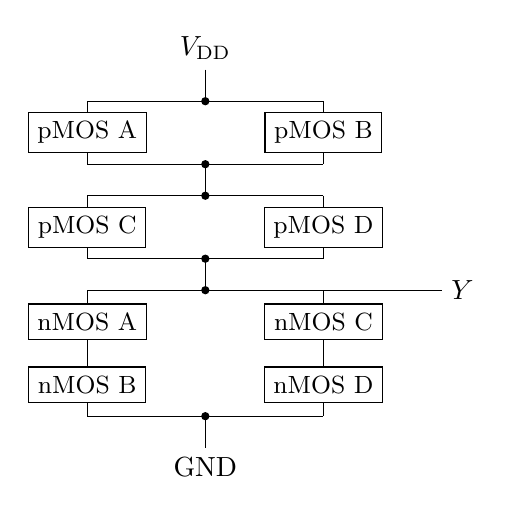
\begin{tikzpicture}[x=1cm,y=0.8cm]
\node[above] at (0,6) {$V_{\mathrm{DD}}$};
\draw (0,6)--(0,5.5)--(-1.5,5.5) (0,5.5)--(1.5,5.5);
\draw (-1.5,5.5)--(-1.5,4.5) node[midway,draw,fill=white,font=\small] {pMOS A};
\draw (1.5,5.5)--(1.5,4.5) node[midway,draw,fill=white,font=\small] {pMOS B};
\draw (-1.5,4.5)--(1.5,4.5);\draw (0,4.5)--(0,4)--(-1.5,4) (0,4)--(1.5,4);
\draw (-1.5,4)--(-1.5,3) node[midway,draw,fill=white,font=\small] {pMOS C};
\draw (1.5,4)--(1.5,3) node[midway,draw,fill=white,font=\small] {pMOS D};
\draw (-1.5,3)--(1.5,3);\draw (0,3)--(0,2.5)--(3,2.5) node[right] {$Y$};
\draw (0,2.5)--(-1.5,2.5)--(-1.5,1.5) node[midway,draw,fill=white,font=\small] {nMOS A};
\draw (0,2.5)--(1.5,2.5)--(1.5,1.5) node[midway,draw,fill=white,font=\small] {nMOS C};
\draw (-1.5,1.5)--(-1.5,0.5) node[midway,draw,fill=white,font=\small] {nMOS B};
\draw (1.5,1.5)--(1.5,0.5) node[midway,draw,fill=white,font=\small] {nMOS D};
\draw (-1.5,0.5)--(1.5,0.5);\draw (0,0.5)--(0,0) node[below] {GND};
\foreach \x/\y in {0/5.5,0/4.5,0/4,0/3,0/2.5,0/0.5} {\fill (\x,\y) circle (1.5pt);}
\end{tikzpicture}
\end{latin}
\caption{نمای توپولوژی آموزشی \lr{AOI22} برای رابطه \eqref{eq:ch1-aoi}.
بلوک‌های برچسب‌دار در این نمایش جایگزین نماد ترانزیستورند؛
وضعیت هدایت هر بلوک به نوع ترانزیستور و ورودی نوشته‌شده در آن بستگی دارد.}
\label{fig:ch1-aoi}
\end{figure}

نام \lr{AND-OR-Invert (AOI22)} می‌گوید دو گروه \lr{AND} دوورودی داریم،
خروجی آن‌ها \lr{OR} و سپس معکوس می‌شود.
در مثال \((A,B,C,D)=(1,1,0,0)\)، شاخه \(AB\) پایین وصل است؛
در بالا گروه \(A,B\) کاملاً قطع است، پس \(Y=0\).
در \((1,0,1,0)\)، هر شاخه پایین یک ترانزیستور قطع دارد؛
در بالا از \(B\) و \(D\) مسیر کامل داریم، پس \(Y=1\).
این دو مثال جای بررسی تمام حالت‌ها را نمی‌گیرند؛ رابطه مکمل، پوشش همه حالت‌ها را می‌دهد.

\textbf{مثال کتاب، \lr{OAI31}.} برای
\(Y=\overline{(A+B+C)D}\)، پایین گروه موازی \(A,B,C\) را با \(D\) سری می‌کنیم.
بالا گروه سری سه \lr{pMOS} با کنترل \(A,B,C\) را با یک \lr{pMOS} کنترل‌شده با \(D\)
موازی می‌کنیم؛ چون شرط بالا
\(\overline{A}\,\overline{B}\,\overline{C}+\overline{D}\) است.
این هشت ترانزیستور، تابع مثال \secnum{۱.۲} کتاب را می‌سازند
\cite[صفحه چاپی ۱۲]{weste}.

\subsection{چرا \lr{AND} را با یک \lr{NAND} و یک \lr{Inverter} می‌سازیم؟}
در خانواده محدود شبکه‌های مکمل ایستا که ورودی‌های غیرمعکوس مستقیماً
\lr{Gate}ها را کنترل می‌کنند، روشن شدن مسیر پایین خروجی را صفر می‌کند؛
ازاین‌رو گیت یک‌مرحله‌ای، تابع معکوس‌کننده ورودی‌هاست.
جابه‌جا کردن ساده \lr{nMOS} و \lr{pMOS} برای ساخت \lr{Buffer} مناسب نیست؛
با انتقال سطوح ضعیف روبه‌رو می‌شویم \cite[صفحه چاپی ۱۴]{weste}.
به‌جای آن، دو معکوس‌سازی می‌دهند
\[
 Y=\overline{\overline{AB}}=AB.
\]
برای \lr{OR} نیز \lr{NOR} و سپس \lr{Inverter} به کار می‌رود.

\lr{AND} دوورودی با این روش شش ترانزیستور دارد: چهار برای \lr{NAND}
و دو برای \lr{Inverter}. ساخت تابع \lr{AOI22} از دو \lr{AND}، یک \lr{OR}
و یک \lr{Inverter} با این سلول‌های ساده، \(6+6+6+2=20\)
ترانزیستور می‌خواهد؛ گیت \lr{Compound} فقط هشت ترانزیستور دارد.
این مقایسه شمارش قطعات است؛ برای نتیجه قطعی درباره \lr{Delay} یا توان باید
اندازه ترانزیستورها، بار و مسیرها نیز تحلیل شوند \cite[شکل \secnum{۱.۲۴}]{weste}.

\subsection{کنترل اعتبار گیت ایستا}
برای هر ترکیب ورودی، ابتدا قطع یا وصل بودن تک‌تک قطعات و سپس وجود مسیر کامل
را مشخص می‌کنیم. اگر پایین هدایت دارد، بالا باید قطع باشد و برعکس.
این کنترل برای تمام ورودی‌ها، شرط منطقی طراحی است.
در مدل ایدئال پایدار، ابعاد ترانزیستورها جدول درستی را عوض نمی‌کنند؛
در مدار واقعی، ابعاد بر زمان و توان و رفتار گذرا اثر دارند.
عبارت «توان ساکن صفر» نیز فقط به مدل بدون نشتی و ورودی‌های پایدار معتبر تعلق دارد؛
بار خازنی و هدایت هم‌زمان در گذار، همچنان انرژی مصرف می‌کنند.

% !TeX root = booklet-01.tex
\section{انتقال داده و خروجی سه‌حالته}
\label{sec:ch1-pass}
\subsection{کنترل مسیر با تولید سطح منطقی فرق دارد}
در گیت ایستای قبلی، ورودی به \lr{Gate}ها می‌رفت و خروجی از ریل تغذیه یا زمین
تولید می‌شد. در \lr{Pass Transistor}، خود داده از مسیر \lr{Source--Drain}
عبور می‌کند؛ \lr{Gate} فقط مسیر عبور را کنترل می‌کند.
این تفاوت توضیح می‌دهد چرا یک کلید روشن الزاماً ولتاژ داده را بدون تغییر عبور نمی‌دهد
\cite[بخش \secnum{۱.۴.۶}]{weste}.

\textbf{مثال آموزشی برای عبور یک.} \lr{nMOS} با \lr{Gate} در
\(V_{\mathrm{DD}}\) گره خروجی را از ولتاژ پایین شارژ می‌کند.
با بالا رفتن خروجی، پایانه کم‌ولتاژ مسیر نیز بالا می‌رود و
\(V_{gs}=V_{\mathrm{DD}}-V_{\mathrm{out}}\) کم می‌شود.
در مدل آستانه ثابت، حد شارژ وقتی است که این اختلاف به \(V_{tn}\) برسد:
\begin{equation}\label{eq:ch1-pass-high}
V_{\mathrm{out,lim}}=V_{\mathrm{DD}}-V_{tn}.
\end{equation}
از رابطه \(V_{\mathrm{DD}}-V_{\mathrm{out}}=V_{tn}\)،
ابتدا \(V_{\mathrm{out}}\) را به طرف دیگر و سپس \(V_{tn}\) را کم کردیم.
برای تغذیه فرضی \(\qty{1}{\volt}\) و آستانه \(\qty{0.3}{\volt}\)،
حد خروجی \(\qty{0.7}{\volt}\) است؛ نه یک ولت.
این حد در مدل بدون نشتی، بدون بار رسانشی و با شروع از ولتاژ پایین بیان شده است.
با \lr{Body Effect}، خود آستانه نیز تغییر می‌کند؛ تحلیل کامل به جزوه سوم تعلق دارد.

\lr{nMOS} در انتقال صفر به زمین چنین افت آستانه‌ای ایجاد نمی‌کند؛
ازاین‌رو کتاب از «صفر قوی و یک ضعیف» صحبت می‌کند.
\lr{pMOS} برعکس، یک را قوی و صفر را با افت انتقال می‌دهد:
با \lr{Gate} صفر، حد دشارژ در مدل مشابه نزدیک \(|V_{tp}|\) است
\cite[شکل \secnum{۱.۲۰}]{weste}.
«ضعیف» یعنی سطح از ریل فاصله دارد و توان راه‌اندازی نیز به شرایط مدار وابسته است؛
این اصطلاح به‌تنهایی تعیین نمی‌کند سطح برای ورودی گیت بعد معتبر است یا خیر.

\subsection{\lr{Transmission Gate}: ترکیب دو نوع مکمل}
با موازی کردن \lr{nMOS} و \lr{pMOS} و اعمال کنترل‌های مکمل،
\lr{Transmission Gate (TG)} می‌سازیم. برای \(E=1\)،
\lr{Gate} ترانزیستور \lr{nMOS} یک و \lr{Gate} ترانزیستور \lr{pMOS}
صفر است؛ مسیر داده فعال می‌شود. برای \(E=0\)، هر دو خاموش‌اند.
در انتقال صفر، \lr{nMOS} و در انتقال یک، \lr{pMOS} سطح مناسب را پشتیبانی می‌کند
\cite[شکل \secnum{۱.۲۱}]{weste}.
شکل \ref{fig:ch1-tg} این موازی بودن را نشان می‌دهد.

\begin{figure}[ht]
\centering
\begin{latin}
\begin{circuitikz}[american]
\draw (0,1) node[pmos,rotate=-90] (p) {};
\draw (0,-1) node[nmos,rotate=90] (n) {};
\draw (p.D)--(-2,1)--(-2,-1)--(n.D);
\draw (p.S)--(2,1)--(2,-1)--(n.S);
\draw (-2,0) to[short,*-o] (-3,0) node[left] {$a$};
\draw (2,0) to[short,*-o] (3,0) node[right] {$b$};
\draw (p.G)--(0,2.2) node[above] {$\overline{E}$};
\draw (n.G)--(0,-2.2) node[below] {$E$};
\node[right] at (0.7,1.5) {pMOS};\node[right] at (0.7,-1.5) {nMOS};
\end{circuitikz}
\end{latin}
\caption{بازترسیم آموزشی \lr{TG} بر پایه کتاب \cite{weste}.
پایانه‌های داده \(a,b\) دو سوی یک مسیر قابل‌کنترل‌اند؛
بدنه \lr{nMOS} به زمین و بدنه \lr{pMOS} به تغذیه متصل است.}
\label{fig:ch1-tg}
\end{figure}

مکمل کنترل رایگان نیست؛ اگر \(\overline{E}\) از قبل موجود نباشد،
یک \lr{Inverter} یا مدار تولید مکمل لازم است.
خود \lr{TG} دو ترانزیستور دارد، اما شمارش کل مدار باید هزینه کنترل را هم در نظر بگیرد.
برچسب \(a,b\) عمدی است؛ جهت انتقال می‌تواند با بایاس عوض شود.
این کاربرد برای ولتاژهای داخل ریل‌های مجاز بررسی می‌شود، نه یک کلید عمومی برای هر ولتاژی.

\subsection{تفاوت \lr{Restoring} و \lr{Nonrestoring}}
یک گیت \lr{Restoring}، سطح ورودی معتبر را با استفاده از تغذیه به خروجی نزدیک
ریل بازتولید می‌کند. مثلاً دو \lr{Inverter} پشت‌سرهم، داده را بدون تغییر منطقی
و با بازسازی سطح عبور می‌دهند؛ محدوده معتبر ورودی باید رعایت شود.
\lr{TG} داده را عبور می‌دهد و نویز یا افت ولتاژ آن را به‌خودی‌خود حذف نمی‌کند؛
بنابراین \lr{Nonrestoring} است \cite[بخش \secnum{۱.۴.۷}]{weste}.
«عبور هر دو سطح ریل» را نباید با «بازسازی ورودی خراب» برابر دانست.
زنجیره‌های بلند مسیر عبوری نیز مقاومت و ظرفیت دارند و در مدل واقعی تاخیرشان افزایش می‌یابد.

\subsection{\lr{Tristate}: مقدار \texorpdfstring{\(Z\)}{Z} یک سطح ولتاژ سوم نیست}
\lr{Tristate Buffer} در حالت فعال \(Y=A\) و در حالت غیرفعال خروجی
\lr{High Impedance} دارد. \(Z\) یعنی مدار خروجی را به‌طور فعال به صفر یا یک
نمی‌کشد؛ یک ولتاژ مشخص میان صفر و تغذیه نیست.
یک \lr{TG} همین جدول منطقی فعال/غیرفعال را دارد، ولی \lr{Restoring} نیست
\cite[صفحات چاپی ۱۴ و ۱۵]{weste}.

\lr{Tristate Inverter} در حالت فعال، خروجی \(\overline{A}\) می‌دهد و در حالت
غیرفعال \(Z\). برای ساخت آن، در مسیر بالایی \lr{Inverter} یک \lr{pMOS}
با کنترل \(\overline{E}\) و در مسیر پایینی یک \lr{nMOS} با کنترل \(E\)
سری می‌کنیم. پس:
\begin{equation}\label{eq:ch1-tristate}
F_{\mathrm{PUN}}=E\overline{A},\qquad
F_{\mathrm{PDN}}=EA.
\end{equation}
اگر \(E=1\)، شبکه‌ها مانند \lr{Inverter} عمل می‌کنند؛ اگر \(E=0\)،
هر دو قطع‌اند. جدول \ref{tab:ch1-tri} نتیجه را نشان می‌دهد.
شماتیک شکل \ref{fig:ch1-tri} محل ترانزیستورهای فعال‌ساز را مشخص می‌کند.

\begin{figure}[ht]
\centering
\begin{latin}
\begin{circuitikz}[american,scale=0.85,transform shape]
\draw (0,4.5) node[pmos] (pe) {} (0,2.7) node[pmos] (pa) {};
\draw (0,-0.3) node[nmos] (na) {} (0,-2.1) node[nmos] (ne) {};
\draw (pe.S)--(0,5.5) node[above] {$V_{\mathrm{DD}}$};
\draw (pe.D)--(pa.S) (pa.D)--(0,1.2)--(na.D) (na.S)--(ne.D);
\draw (ne.S)--(0,-3.1) node[ground] {};
\draw (0,1.2) to[short,*-o] (2,1.2) node[right] {$Y$};
\node[left] at (pe.G) {$\overline{E}$};\node[left] at (pa.G) {$A$};
\node[left] at (na.G) {$A$};\node[left] at (ne.G) {$E$};
\end{circuitikz}
\end{latin}
\caption{بازترسیم آموزشی \lr{Tristate Inverter} بر پایه شکل \secnum{۱.۲۷} کتاب
\cite{weste}. برچسب‌های یکسان \lr{Gate} یعنی ورودی مشترک؛
بدنه‌های \lr{pMOS} به تغذیه و \lr{nMOS} به زمین متصل‌اند.}
\label{fig:ch1-tri}
\end{figure}

\begin{table}[ht]
\centering
\caption{جدول \lr{Tristate Inverter}؛ مکمل کنترل در شمارش قطعات فرض نشده است.}
\label{tab:ch1-tri}
\begin{tabular}{ccc}
\toprule
\(E\)&\(A\)&\(Y\)\\
\midrule
۰&۰&\(Z\)\\
۰&۱&\(Z\)\\
۱&۰&۱\\
۱&۱&۰\\
\bottomrule
\end{tabular}
\end{table}
هسته این مدار چهار ترانزیستور دارد و خروجی فعالش \lr{Restoring} است.
برای \lr{Tristate Buffer} می‌توان یک \lr{Inverter} عادی پیش از آن گذاشت تا
دو معکوس‌سازی یکدیگر را خنثی کنند.

اگر چند فرستنده به یک \lr{Bus} وصل شوند، باید قرارداد فعال‌سازی مانع فرمان‌های
متضاد شود. دو فرستنده فعال با داده مخالف، \lr{Contention} ایجاد می‌کنند؛
نبود هیچ فرستنده فعال نیز می‌تواند \lr{Bus} را شناور کند.
حتی اگر دو داده در یک لحظه یکسان باشند، فعال‌سازی هم‌زمان درستی پروتکل را تضمین نمی‌کند.
تاخیر مسیرهای کنترل ممکن است هنگام جابه‌جایی فرستنده‌ها، هم‌پوشانی موقت بسازد؛
ازاین‌رو جایگزینی با \lr{Multiplexer} در بسیاری از طراحی‌ها مفید است
\cite[بخش \secnum{۱.۴.۷}]{weste}.

\section{\lr{Multiplexer}: انتخاب یکی از چند ورودی}
\label{sec:ch1-mux}
\subsection{از تعریف انتخاب تا رابطه منطقی}
\lr{Multiplexer} یا \lr{MUX} دوورودی، با انتخاب \(S=0\) داده \(D_0\)
و با \(S=1\) داده \(D_1\) را به خروجی می‌فرستد. بنابراین:
\begin{equation}\label{eq:ch1-mux}
Y=\overline{S}D_0+SD_1.
\end{equation}
وقتی \(S=0\)، جمله دوم صفر و جمله اول \(D_0\) است؛ وقتی \(S=1\)،
جمله اول صفر و جمله دوم \(D_1\). این جای‌گذاری ساده، هم رابطه و هم جهت انتخاب
را کنترل می‌کند \cite[بخش \secnum{۱.۴.۸}]{weste}.
زیرنویس‌های صفر و یک بخشی از نام دو ورودی‌اند؛ ضرب در صفر یا یک نیستند.

\subsection{پیاده‌سازی با دو \lr{TG}}
دو \lr{TG} را از \(D_0\) و \(D_1\) به گره مشترک \(Y\) وصل می‌کنیم.
کنترل فعال‌ساز مسیر اول \(\overline{S}\) و مسیر دوم \(S\) است.
برای هر مسیر، ترانزیستور \lr{nMOS} همان کنترل فعال‌ساز و \lr{pMOS} مکمل آن
را می‌گیرد. در مدل کنترل‌های مکمل ایدئال، دقیقاً یک مسیر باز است.
شکل \ref{fig:ch1-mux} نمای بلوکی همین اتصال را نشان می‌دهد.

\begin{figure}[ht]
\centering
\begin{latin}
\begin{tikzpicture}[x=1.2cm,y=1cm]
\node[draw,minimum width=1.8cm,minimum height=0.8cm] (t0) at (0,1.2) {TG};
\node[draw,minimum width=1.8cm,minimum height=0.8cm] (t1) at (0,-1.2) {TG};
\draw[->] (-2.2,1.2) node[left] {$D_0$}--(t0.west);
\draw[->] (-2.2,-1.2) node[left] {$D_1$}--(t1.west);
\draw (t0.east)--(2,1.2)--(2,-1.2)--(t1.east);
\draw[->] (2,0)--(3.1,0) node[right] {$Y$};\fill (2,0) circle (1.5pt);
\draw[->] (0,2.4) node[above] {$E_0=\overline{S}$}--(t0.north);
\draw[->] (0,-2.4) node[below] {$E_1=S$}--(t1.south);
\end{tikzpicture}
\end{latin}
\caption{نمای بلوکی آموزشی \lr{MUX} بر پایه شکل \secnum{۱.۲۸} کتاب \cite{weste}.
هر بلوک \lr{TG} شامل دو ترانزیستور شکل \ref{fig:ch1-tg} است؛
پیکان کنترل مسیر داده نیست.}
\label{fig:ch1-mux}
\end{figure}

هسته \lr{MUX} دو \lr{TG}، چهار ترانزیستور دارد؛ با تولید محلی
\(\overline{S}\) به کمک یک \lr{Inverter}، تعداد به شش می‌رسد.
این مدار \lr{Nonrestoring} است. قرار دادن \lr{Inverter} در خروجی،
سطح را بازسازی می‌کند ولی تابع را معکوس می‌کند؛ برای خروجی غیرمعکوس بازسازی‌شده،
به دو معکوس‌سازی یا پیاده‌سازی مناسب دیگری نیاز داریم.

در پیاده‌سازی گیتی، دو \lr{Tristate Inverter} با فعال‌سازهای مکمل
می‌توانند خروجی مشترک \(\overline{Y}\) را بسازند.
روش دیگر، گیت \lr{AOI22} با ورودی‌های \(\overline{S},D_0,S,D_1\) است.
کتاب این پیاده‌سازی‌ها را مقایسه می‌کند؛ استفاده از مکمل بودن دو کنترل،
گاهی اجازه ساده‌سازی شبکه را می‌دهد \cite[شکل \secnum{۱.۲۹}]{weste}.
این ساده‌سازی به قید کنترل‌ها متکی است و برای چهار ورودی مستقل قابل تعمیم نیست.

\subsection{انتخاب چهار داده و معنای دو بیت انتخاب}
یک \lr{MUX} چهارورودی را با سه \lr{MUX} دوورودی می‌سازیم.
در مرحله اول، یکی از \(D_0,D_1\) و یکی از \(D_2,D_3\) با \(S_0\)
انتخاب می‌شوند؛ در مرحله دوم، \(S_1\) یکی از دو نتیجه را انتخاب می‌کند.
به‌ترتیب برای \((S_1,S_0)=(0,0),(0,1),(1,0),(1,1)\)،
خروجی \(D_0,D_1,D_2,D_3\) است. شماره ورودی برابر \(2S_1+S_0\) می‌شود.
این ساختار دو مرحله مسیر داده دارد؛ نام چهارورودی به معنی چهار گیت سری نیست.

روش دیگر، چهار مسیر سه‌حالته با فعال‌سازهای
\(\overline{S_1}\overline{S_0}\)، \(\overline{S_1}S_0\)،
\(S_1\overline{S_0}\) و \(S_1S_0\) است
\cite[شکل \secnum{۱.۳۰}]{weste}.
برای ورودی پایدار دقیقاً یکی فعال است؛ کنترل گذرا همچنان باید مانع وصل هم‌زمان
مسیرهای داده متضاد شود. مدل منطقی به‌تنهایی زمان‌بندی واقعی کنترل‌ها را اثبات نمی‌کند.

\subsection{پرسش‌های انتقال و انتخاب}
\begin{enumerate}
\item \textbf{چرا یک \lr{nMOS} با کنترل یک، همیشه یک کامل عبور نمی‌دهد؟}
با بالا رفتن خروجی، اختلاف \(V_{gs}\) کم می‌شود و شرط هدایت از دست می‌رود.
\item \textbf{آیا \(Z\) همان صفر منطقی است؟}
خیر؛ به معنی نداشتن راه‌اندازی فعال است. یک خازن شناور می‌تواند برای مدتی یک قبلی را نگه دارد.
\item \textbf{آیا \lr{TG} نویز ورودی را حذف می‌کند؟}
خیر؛ عبوری و \lr{Nonrestoring} است. بازسازی به یک مدار دارای بهره و تغذیه مناسب نیاز دارد.
\item \textbf{در \lr{MUX} با \(S=1\)، تغییر \(D_0\) چه اثری بر خروجی منطقی دارد؟}
در مدل پایدار اثری ندارد؛ مسیر انتخاب‌شده \(D_1\) است. کوپل خازنی و گذرا در این حکم مدل نشده‌اند.
\end{enumerate}

% !TeX root = booklet-01.tex
\section{ساخت حافظه یک‌بیتی از گیت‌ها}
\label{sec:ch1-storage}
\subsection{چرا \lr{Feedback} لازم می‌شود؟}
خروجی مدار \lr{Combinational} پس از پایدارشدن، تابع ورودی جاری است؛
برای حفظ یک داده قدیمی باید اثری از حالت قبلی در مدار باقی بماند.
در ساختار ایستای این بخش، \lr{Feedback} خروجی را از مسیر گیت‌ها به ورودی برمی‌گرداند.
دو \lr{Inverter} پشت‌سرهم در حلقه، از نظر منطقی دو حالت سازگار دارند:
اگر یک گره صفر باشد، گره دیگر یک و بازگشت دوباره صفر است؛ حالت معکوس نیز ممکن است
\cite[بخش \secnum{۱.۴.۹}]{weste}.
این استدلال منطقی، زمان راه‌اندازی، نویز یا \lr{Metastability} را تحلیل نمی‌کند.
حالت اولیه بدون نوشتن داده یا مدار مقداردهی، لزوماً از پیش معلوم نیست.

\subsection{\lr{D Latch} با \lr{MUX} و دو \lr{Inverter}}
در شکل \ref{fig:ch1-latch}، یک \lr{MUX} بین ورودی تازه \(D\) و بازگشت
خروجی \(Q\) انتخاب می‌کند. پس از \lr{MUX} دو \lr{Inverter} داریم؛
آن‌ها سطح را بازسازی می‌کنند و مجموع اثر منطقی‌شان غیرمعکوس است.
برای \(E=1\)، ورودی تازه انتخاب و برای \(E=0\)، بازخورد انتخاب می‌شود
\cite[شکل \secnum{۱.۳۱}]{weste}.

\begin{figure}[ht]
\centering
\begin{latin}
\begin{tikzpicture}[x=1cm,y=1cm]
\draw (0,0)--(0,2)--(1.2,1.7)--(1.2,0.3)--cycle;
\node at (0.55,1.35) {$D$};\node at (0.55,0.65) {$Q$};
\draw[->] (-1.4,1.4) node[left] {$D$}--(0,1.4);
\draw (1.2,1)--(2,1);
\draw (2,0.6)--(2,1.4)--(2.7,1)--cycle;\draw (2.78,1) circle (0.08);
\draw (2.86,1)--(3.5,1);
\draw (3.5,0.6)--(3.5,1.4)--(4.2,1)--cycle;\draw (4.28,1) circle (0.08);
\draw[->] (4.36,1)--(5.9,1) node[right] {$Q$};
\draw (5.1,1)--(5.1,-1)--(-0.8,-1)--(-0.8,0.6)--(0,0.6);
\fill (5.1,1) circle (1.5pt);
\draw[->] (0.6,3) node[above] {$E$}--(0.6,1.85);
\node at (0.5,2.3) {MUX};
\node[above] at (2.9,1.2) {$\overline{Q}$};
\end{tikzpicture}
\end{latin}
\caption{بازترسیم بلوکی \lr{Latch} مثبت‌حساس بر پایه کتاب \cite{weste}.
در \lr{MUX}، \(E=1\) ورودی \(D\) و \(E=0\) بازخورد \(Q\) را انتخاب می‌کند.
نام گره میانی \(\overline{Q}\) معنای منطقی پایدار آن را نشان می‌دهد.}
\label{fig:ch1-latch}
\end{figure}

رابطه حالت در مدل منطقی چنین است:
\begin{equation}\label{eq:ch1-latch}
Q_{\mathrm{next}}=ED+\overline{E}Q_{\mathrm{current}}.
\end{equation}
برای \(E=1\)، رابطه به \(Q_{\mathrm{next}}=D\) تبدیل می‌شود؛
تا وقتی فعال‌ساز یک است، خروجی پس از تاخیرهای مدار تغییر ورودی را دنبال می‌کند.
این حالت \lr{Transparent} است؛ \lr{Latch} فقط در لحظه بالا رفتن \(E\) نمونه نمی‌گیرد.
برای \(E=0\)، داده تازه جدا و حلقه بازخورد بسته می‌شود؛
رابطه به \(Q_{\mathrm{next}}=Q_{\mathrm{current}}\) تبدیل می‌شود و داده حفظ می‌شود.
به این حالت \lr{Opaque} می‌گوییم.

در پیاده‌سازی \lr{TG}، مسیر ورودی با \(E\) و مسیر بازخورد با \(\overline{E}\)
فعال می‌شود؛ دو کنترل مکمل باید هر دو مسیر را هماهنگ کنند.
با دو \lr{TG} و دو \lr{Inverter}، هسته هشت ترانزیستور دارد؛
این شمارش تولید مکمل کنترل و مدارهای جانبی را شامل نمی‌شود.
وجود دو \lr{Inverter} باعث می‌شود نگهداری صرفاً به بار یک خازن جداافتاده متکی نباشد؛
در مدل ایستای تغذیه‌شده، بازخورد حالت را بازتولید می‌کند.

\subsection{جدول زمانی آموزشی برای \lr{Latch}}
جدول \ref{tab:ch1-latch-time} یک توالی مستقل آموزشی است.
حالت اولیه صفر فرض شده و میان رویدادها زمان کافی برای پایدار شدن داریم.
\begin{table}[ht]
\centering
\caption{ردگیری یک \lr{Latch} مثبت‌حساس؛ هر ردیف وضعیت پس از رویداد را نشان می‌دهد.}
\label{tab:ch1-latch-time}
\begin{tabular}{cccp{7cm}}
\toprule
\(E\)&\(D\)&\(Q\)&توضیح\\
\midrule
۰&۰&۰&حالت اولیه فرض‌شده نگه داشته می‌شود.\\
۱&۰&۰&مسیر داده باز می‌شود؛ خروجی صفر است.\\
۱&۱&۱&بدون لبه تازه فعال‌ساز، تغییر داده عبور می‌کند.\\
۰&۱&۱&مسیر داده بسته و یک نگه داشته می‌شود.\\
۰&۰&۱&داده تغییر کرده است؛ خروجی نگه داشته می‌شود.\\
\bottomrule
\end{tabular}
\end{table}
این جدول تفاوت حساسیت به سطح و حساسیت به لبه را نشان می‌دهد.
با عوض کردن ورودی‌های \lr{MUX}، می‌توان \lr{Latch} منفی‌حساس ساخت:
آن‌گاه وقتی کنترل صفر است شفاف و وقتی یک است نگهدارنده خواهد بود.

\subsection{\lr{D Flip-Flop} از دو \lr{Latch} مکمل}
یک \lr{Latch} منفی‌حساس را \lr{Master} و پس از آن یک \lr{Latch}
مثبت‌حساس را \lr{Slave} قرار می‌دهیم.
هر دو از همان \lr{Clock} به نام \(CLK\) استفاده می‌کنند، ولی فعال‌ساز
اولی \(\overline{CLK}\) و دومی \(CLK\) است
\cite[شکل \secnum{۱.۳۲}]{weste}.
شکل \ref{fig:ch1-flop} مسیر داده را نشان می‌دهد.

\begin{figure}[ht]
\centering
\begin{latin}
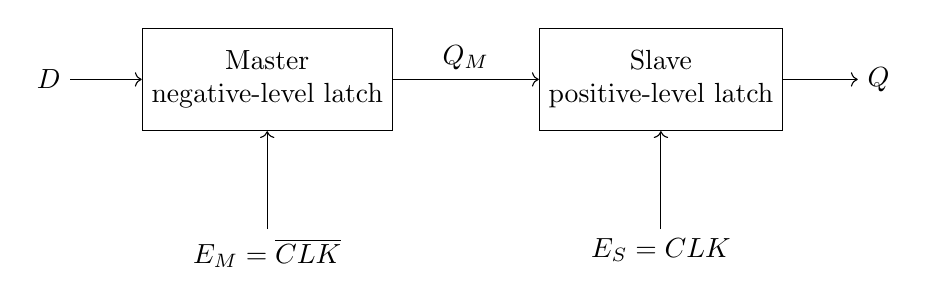
\begin{tikzpicture}[x=1cm,y=1cm]
\node[draw,minimum width=2.8cm,minimum height=1.3cm,align=center] (m) at (0,0)
{Master\\negative-level latch};
\node[draw,minimum width=2.8cm,minimum height=1.3cm,align=center] (s) at (5,0)
{Slave\\positive-level latch};
\draw[->] (-2.5,0) node[left] {$D$}--(m.west);
\draw[->] (m.east)--node[above] {$Q_M$} (s.west);
\draw[->] (s.east)--(7.5,0) node[right] {$Q$};
\draw[->] (0,-1.9) node[below] {$E_M=\overline{CLK}$}--(m.south);
\draw[->] (5,-1.9) node[below] {$E_S=CLK$}--(s.south);
\end{tikzpicture}
\end{latin}
\caption{ساختار آموزشی \lr{Master--Slave Flip-Flop} لبه‌بالارونده.
هر بلوک یک \lr{Latch} است؛ پیکان‌های پایین فقط کنترل شفاف بودن‌اند.}
\label{fig:ch1-flop}
\end{figure}

سه وضعیت را جدا بررسی می‌کنیم:
\begin{enumerate}
\item \textbf{هنگام صفر بودن \lr{Clock}:}
\lr{Master} شفاف است و \(Q_M\) داده \(D\) را دنبال می‌کند؛
\lr{Slave} بسته است و خروجی قبلی \(Q\) را نگه می‌دارد.
پس تغییر \(D\) در این فاز فوراً به \(Q\) نمی‌رسد.
\item \textbf{در گذار صفر به یک:}
\lr{Master} بسته و مقدار داده نزدیک این لبه را نگه می‌دارد؛
\lr{Slave} باز می‌شود و آن مقدار ذخیره‌شده را به \(Q\) می‌رساند.
پس از تاخیر انتشار، خروجی با نمونه ثبت‌شده برابر می‌شود.
\item \textbf{هنگام یک بودن و سپس افت \lr{Clock}:}
در فاز یک، تغییر بعدی \(D\) از \lr{Master} بسته عبور نمی‌کند.
در لبه افت، \lr{Slave} بسته و خروجی را نگه می‌دارد؛
\lr{Master} دوباره برای نمونه بعدی باز می‌شود.
\end{enumerate}
در مدل ایدئال، این رفتار با ثبت \(D\) در لبه بالارونده معادل است؛
دو \lr{Latch} هم‌حساس چنین جداسازی فازهایی ندارند و ممکن است مسیر شفاف سرتاسری بسازند.
با جابه‌جا کردن قطبیت دو \lr{Latch}، \lr{Flip-Flop} لبه‌پایین‌رونده ساخته می‌شود.

\subsection{نمونه‌برداری لبه‌ای، حالت اولیه و محدودیت زمانی}
فرض کنید \(Q\) ابتدا صفر است و \(D\) پیش از لبه اول یک شده و پیرامون لبه
پایدار می‌ماند. در لبه اول، خروجی پس از تاخیر انتشار یک می‌شود.
اگر \(D\) میان دو لبه به صفر برسد، خروجی تا لبه بعدی یک می‌ماند؛
به شرط رعایت محدودیت‌های زمانی، در لبه بعدی صفر ثبت می‌شود.
بدون تعیین داده ثبت‌شده یا مقداردهی اولیه، \(Q\) را نباید خودبه‌خود صفر فرض کرد.

در مدار واقعی، داده باید پیش از لبه برای مدت \lr{Setup Time} و پس از آن برای
مدت \lr{Hold Time} پایدار بماند. این اصطلاح‌ها به پنجره اطمینان ثبت مربوط‌اند؛
نقضشان ممکن است خروجی نامطمئن ایجاد کند.
\lr{Clock Skew} اختلاف زمان رسیدن ساعت به عناصر مختلف است و می‌تواند
شرایط نگهداری را تحت تاثیر قرار دهد \cite[ابتدای صفحه چاپی ۱۹]{weste}.
این بخش مقدار عددی هیچ‌یک را تعیین یا بی‌خطا بودن زمان‌بندی یک مدار واقعی را اثبات نمی‌کند.

\subsection{دو فاز غیرهم‌پوشان و \lr{Register}}
کتاب برای کاهش خطر شفاف بودن هم‌زمان مسیرهای دو مرحله، ساختاری با دو فاز
\(\phi_1\) و \(\phi_2\) غیرهم‌پوشان معرفی می‌کند
\cite[شکل \secnum{۱.۳۳}]{weste}.
منظور از غیرهم‌پوشان این است که دو فعال‌ساز هم‌زمان یک نباشند؛
میان آن‌ها می‌تواند فاصله‌ای باشد که هر دو صفرند.
در مدل \lr{Latch}، بنابراین دست‌کم یک مرحله بسته می‌ماند و مسیر شفاف کامل نداریم.
این نتیجه به حفظ قید غیرهم‌پوشانی در محل دریافت کنترل‌ها وابسته است؛
جای تحلیل همه محدودیت‌های واقعی و \lr{Setup Time} را نمی‌گیرد.

چند \lr{D Flip-Flop} با \lr{Clock} مشترک، یک \lr{Register} چندبیتی می‌سازند.
برای مثال، هشت \lr{Flip-Flop}، برداری هشت‌بیتی را در لبه ساعت ثبت می‌کنند.
وجود یک \lr{Clock} منطقی مشترک به معنی صفر بودن اختلاف تاخیر مسیرهای ساعت نیست.
بافرگذاری ورودی و خروجی برای ایجاد رابط مناسب میان ماژول‌ها نیز در پایان
بحث کتاب مطرح شده است؛ جزئیات \lr{Modularity} در ادامه فصل می‌آید.

\section{تمرین‌های تحلیلی و کنترل پوشش}
\subsection{پرسش‌ها}
\begin{enumerate}
\item چرا دو برابر شدن تعداد ترانزیستورها به معنی نصف شدن تاخیر هر مدار نیست؟
\item برای \(Y=\overline{A(B+C)}\)، شبکه بالا و پایین را تعیین و تعداد قطعات را بشمارید.
\item در \lr{AOI22} با \((A,B,C,D)=(0,1,1,1)\)، کدام مسیر خروجی را تعیین می‌کند؟
\item در یک \lr{MUX} دوورودی با \(D_0=1,D_1=0\)، تابع خروجی نسبت به \(S\) چیست؟
\item در \lr{Latch} مثبت‌حساس، اگر داده هنگام صفر بودن کنترل تغییر کند، خروجی چه می‌شود؟
\item آیا با سری کردن دو \lr{Latch} مثبت‌حساس با کنترل مشترک،
همان \lr{Flip-Flop} لبه‌ای قبلی را به دست می‌آوریم؟
\end{enumerate}

\subsection{پاسخ‌های تشریحی}
\begin{enumerate}
\item شمار ترانزیستور، مشخصه ساختار است؛ تاخیر به مسیر، جریان، ظرفیت، سیم‌ها و بار وابسته است.
مدل رشد تعداد به‌تنهایی هیچ‌یک از این وابستگی‌ها را حل نمی‌کند.
\item پایین، \lr{nMOS} کنترل‌شده با \(A\) را با گروه موازی \(B,C\) سری می‌کنیم.
بالا، \lr{pMOS} کنترل‌شده با \(A\) را با گروه سری \(B,C\) موازی می‌کنیم؛
شرط بالا \(\overline{A}+\overline{B}\,\overline{C}\) است.
سه ترانزیستور در هر شبکه و مجموعاً شش ترانزیستور داریم.
\item شاخه \(CD\) پایین کامل است؛ خروجی صفر می‌شود.
در بالا گروه \(C,D\) کاملاً قطع است، پس مسیر متضاد نداریم؛ روشن بودن بخشی از شبکه بالا کافی نیست.
\item از رابطه \eqref{eq:ch1-mux}، \(Y=\overline{S}\) به دست می‌آید.
برای \(S=0\)، ورودی اول یک و برای \(S=1\)، ورودی دوم صفر انتخاب می‌شود.
\item مسیر ورودی تازه قطع است و حلقه بازخورد مقدار قبلی را نگه می‌دارد؛
اگر حالت اولیه معلوم نباشد، از این رویداد به‌تنهایی مقدار خروجی معلوم نمی‌شود.
\item خیر؛ در فاز یک، هر دو شفاف‌اند و داده می‌تواند از هر دو عبور کند.
ساختار معرفی‌شده به قطبیت مکمل دو مرحله و زمان‌بندی مناسب نیاز دارد.
\end{enumerate}

\subsection{آنچه اکنون باید بتوانید توضیح دهید}
بخش \secnum{۱.۱} رشد مجتمع‌سازی و محدودیت تفسیر آمار تاریخی را معرفی کرد؛
بخش \secnum{۱.۲} مسیر تابع تا مدار و شکل فیزیکی را نشان داد؛
بخش \secnum{۱.۳} ساختار و مدل مقدماتی \lr{MOS} را توضیح داد.
در بخش \secnum{۱.۴} همه زیربخش‌ها از \lr{Inverter} تا گیت‌های
\lr{Compound}، مسیرهای عبوری، \lr{Tristate}، \lr{MUX} و عناصر حافظه بررسی شدند.

برای تحلیل یک مدار تازه، نوع قطعات، کنترل‌ها، مسیر داده و شرایط مدل را جدا بنویسید.
سپس برای ورودی‌های موردنظر مسیر کامل تا هر ریل را دنبال و وجود خروجی شناور یا
هدایت متضاد را کنترل کنید. در عنصر حافظه‌دار، حالت قبلی و فاز کنترل نیز لازم‌اند.
این روش از جدول درستی فراتر می‌رود و زمینه ورود به \lr{Fabrication}، \lr{Layout}
و مدل کمی ترانزیستور را فراهم می‌کند.

\begin{thebibliography}{9}
\bibitem{weste}
\begin{latin}
Neil H. E. Weste and David Money Harris,
\textit{CMOS VLSI Design: A Circuits and Systems Perspective},
Fourth Edition, Pearson, 2011.
\end{latin}
بخش \secnum{۱.۱}: صفحات چاپی ۱ تا ۶؛ بخش \secnum{۱.۲}: صفحه ۶؛
بخش \secnum{۱.۳}: صفحات ۶ تا ۸؛ بخش \secnum{۱.۴}: صفحات ۹ تا ابتدای ۱۹.
در این محدوده، شماره صفحه فایل \lr{PDF} برابر شماره چاپی به‌اضافه ۲۷ است.
شکل‌های اصلی مرتبط عبارت‌اند از \secnum{۱.۹} تا \secnum{۱.۳۳}؛
شماره شکل‌های داخل این جزوه مستقل از کتاب است.
\bibitem{intro}
اسلایدهای محلی \lr{Introduction}، فایل \lr{00-introduction.pdf}:
اسلایدهای ۴ تا ۱۲ برای تاریخچه و رشد، ۱۵ تا ۲۰ برای مقدمه سطوح طراحی،
و ۲۱ تا ۲۷ برای مدل \lr{Switch} و گیت‌ها.
مطابق اسلاید ۲، اصل یادداشت‌ها متعلق به \lr{David Money Harris}، سال ۲۰۱۱،
و نسخه محلی اقتباس‌شده است. شماره اسلاید با صفحه فایل یکسان است.
\bibitem{mos}
اسلایدهای محلی \lr{MOSFET Transistors}، فایل \lr{01-MOSFET Ch2.pdf}،
اسلایدهای ۲ تا ۸ برای مقدمات ساختار و تشکیل کانال؛
اسلایدهای ۱۰ تا ۱۳ برای معنای اختلاف ولتاژهای کنترل.
این ارجاع‌ها مقدمه فصل دوم‌اند؛ استخراج روابط جریان در بخش بعدی جزوه اول انجام می‌شود.
\end{thebibliography}
\end{document}
